\chapter{Background}\label{C:background}

A literature research was performed to inform design decision made in this project, and to evaluate any existing research. It will discuss buck converter design factors and topologies, as well as the various different methods of PWM generation. In performing this literature research, the following terms were used to search for articles from Google Scholar, Engineering Village, and Te Waharoa:

\begin{itemize}
    \item Frequency Variable PWM
    \item Frequency-PWM converter
    \item Switching Frequency Converter
\end{itemize}

These searches returned no research relevant to the designs of this project, with the only related work focusing on the electromagnetic noise reduction using randomised frequency modulation \cite{Roman2001,Familiant2016}. Because of this, research was instead performed to inform the design of the buck converter and the generation of PWM signals.

\section{PWM Generation}\label{S:PWM}

\begin{itemize}

    \item
          Discuss what PWM is, and how it is used in the context of a buck converter.

    \item
          Discuss the different methods of PWM generation.

          \begin{itemize}
              \item Analogue
              \item Digital (Microcontroller \& FPGA)
          \end{itemize}

    \item
          Discuss how PWM is used in the context of the project. Quickly overview how in this project it will be important to modulate both the PWM frequency, and the PWM duty cycle.

\end{itemize}


\section{Buck Converters}\label{S:buck}

The buck converters is a variant of a switch mode power supply that steps down a DC input voltage to a DC output voltage. They are commonly used in a wide variety of consumer and professional appliances such as laptops, phones, and chargers due to their high efficiency compared to other DC-to-DC step down converters such as linear regulators \cite{Mohan2012}.\\

The basic operational components of a buck converter can be seen below in Figure \ref{F:buck_func}. From this we see that a buck converter has three main elements, the input voltage source, two switching components, and an output filter across the load. In the case of Figure \ref{F:buck_func}, the first switching component is an actively controlled switch such as a MOSFET or transistor, and the second a passive switching diode. This configuration of an active and a passive switch is known as the non-synchronous buck converter topology, if the passive diode were to be replaced with a second active switch the topology would be considered synchronous. Although both topologies function under the same fundamental principles, the non-synchronous topology is easier to implement with the drawback of higher losses and therefor lower efficiency.\\

It can also be seen from Figure \ref{F:buck_func} that a buck converter has two operating states that are controlled through the activation of these switching components. By toggling these switching components at high speed though the use of PWM, we can control the current flowing through the inductor of the output filter. By controlling this current we are also able to directly control the current through, and voltage across the output load of the converter. Using this, buck converters will often have a feedback control system in their design to be able to actively control and regulate the output voltage during usage. This controller will vary the duty cycle of the the switching PWM signal, thereby varying the output voltage of the buck converter as shown in Equation \ref{E:V_out}\\

\begin{figure}[H]
      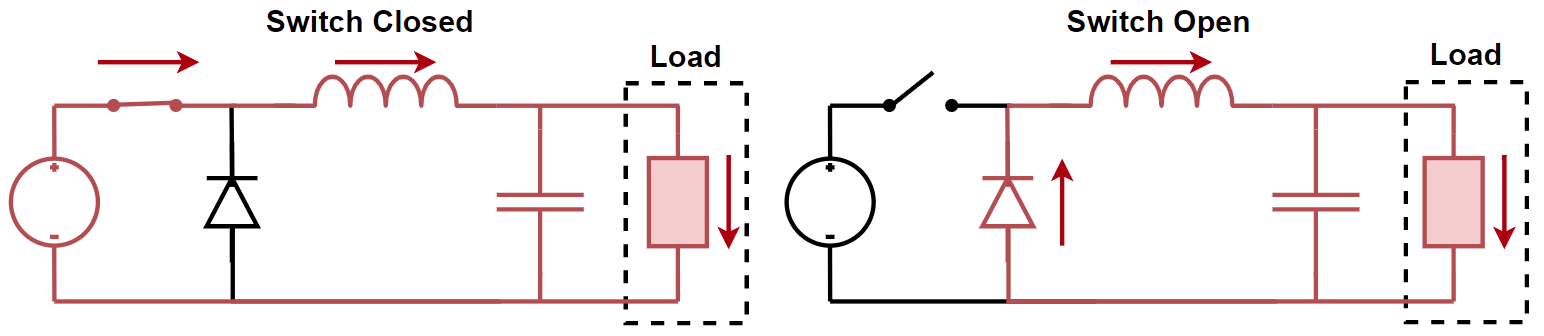
\includegraphics[width = 1\textwidth]{Buck_Functionality.png}
      \caption{Operating states of a buck converter}
      \label{F:buck_func}
  \end{figure}


\subsection{Buck Converter Design}

The design of a common buck converter has two main considerations, the output voltage of the converter $V_0$, and the inductor current ripple of the converter $\Delta i_L$. These considerations can be specified by designing the buck converter using Equation \ref{E:V_out} \& Equation \ref{E:delta_i}.\\ 

When designing a buck converter the first design specification that must be met is the output voltage. In Equation \ref{E:V_out} the output voltage can be directly related to the input voltage $V_{in}$ and the switching duty cycle $D$. Using this equation it is possible to directly set the output voltage of the buck converter by varying this duty cycle.

\begin{align}\label{E:V_out}
      V_o &= D \cdot V_{in}
\end{align}



\begin{align}\label{E:delta_i}
   \Delta i_L &= \frac{ V_{o} \cdot \left( 1 - D \right) } {L \cdot f_s}
\end{align}


\section{Control Systems}\label{S:control}

Possibly not needed in this report as I have not designed any control systems yet for this project?

\begin{itemize}

    \item
          Discuss in very general terms what a control system is what what it seeks to do in a system.

    \item
          Discuss what the control system will be doing in the case of this project. Talk about how a controller will be used to control both the output voltage of the converter, and the inductor ripple of the converter.

\end{itemize}